\section{Soluciones a Atascos}

\subsection{Soluciones a riesgos estructurales}

La solución es simple, se debe replicar, segmentar o realizar turnos para el acceso a las unidades funcionales en conflicto.

\begin{itemize}
  \item Duplicación de recursos de hardware.
  \subitem{Sumadores o restadores además de la ALU.}
  \item Separación en memorias de instrucciones y datos.
  \item Turnar el acceso al banco de registro.
  \subitem{Escrituras en la primera mitad del ciclo de reloj.}
  \subitem{Lecturas en la segunda mitad del ciclo de reloj.}
\end{itemize}

\subsection{Soluciones a riesgos de datos}

Para riesgos \textbf{RAW} se debe determinar cómo y cuando aparecen esos riesgos. Para ello será necesario una unidad de detección de riesgos y/o un compilador más complejo.

Para este tipo de riesgo tenemos dos soluciones:

\begin{itemize}
  \item \textbf{Hardware}
  \subitem{Adelantamiento de operandos (Forwarding).}
  \item \textbf{Software}
  \subitem{Instrucciones NOP o reordenamiento de de codigo.}
\end{itemize}

\subsubsection{Adelantamiento de operandos (Forwarding)}

Esta técnica consiste en pasar directamente el resultado obtenido con una instrucción a las instrucciones que lo necesitan como operando. Si el dato necesario está disponible a la salida de la ALU ($X_i$) se lleva a la entrada de la etapa correspondiente ($X_{i+1}$) sin esperar a la escriturar ($M_i$ o $W_i$).

\begin{figure}[H]
  \centering
  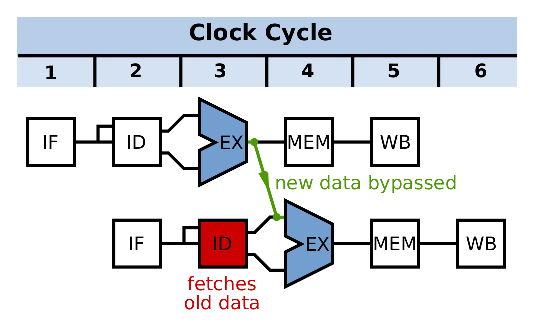
\includegraphics[width=0.7\textwidth]{Forwarding}
  \caption{Adelantamiento de operandos.} 
\end{figure}

\subsubsection{Instrucciones NOP o reordenamiento de código}

Evita los riesgos reordenando las instrucciones del código sin afectar el código. El compilador es el encargado de realizar esta tarea.

Aquí se introducen las instrucciones NOP, que son utilizadas para generar un retardo. Estas instrucciones no realizan ninguna operación, pero consumen un ciclo de reloj. Ademas, se reordenan instrucciones para evitar riesgos RAW.\@

\subsection{Soluciones a riesgos de control}

En los riesgos de control se introduce la penalización por salto. Cuando el salto es incondicional, la dirección de destino se debe determinar lo más pronto posible, dentro del cauce, para reducir la penalización. Cuando el salto es condicional, la penalización se debe a que el procesador no sabe si se debe tomar o no el salto hasta que se evalúe la condición.

Se utiliza una modificación sencilla de la ruta de datos para reducir la cantidad de paradas a un solo ciclo:

\begin{itemize}
  \item \textbf{Adelantar la resolución de los saltos a la etapa D}
  \begin{itemize}
    \item En ella se decodifica y se sabe que es un salto.
    \item Se puede evaluar la condición de salto.
    \item Se puede calcular la dirección de destino.
  \end{itemize}
\end{itemize}

\subsubsection{Técnicas de predicción de salto (Hardware)}

Para este tipo de técnicas tenemos dos posibilidades:

\begin{itemize}
  \item \textbf{Predicción estática}
  \subitem{Se asume que el salto se toma o no se toma.}
  \item \textbf{Predicción dinámica}
  \subitem{Se utiliza un predictor de saltos.}
\end{itemize}

\subsubsection*{Predicción estática}

\begin{itemize}
  \item \textbf{Predicción de salto tomado}
  \subitem{Se asume que el salto se toma.}
  \subitem{Se adelanta la búsqueda de la dirección de destino.}
  \item \textbf{Predicción de salto no tomado}
  \subitem{Se asume que el salto no se toma.}
  \subitem{Se continúa con la ejecución secuencial.}
\end{itemize}

\subsubsection*{Predicción dinámica}

\begin{itemize}
  \item \textbf{Conmutador saltar/no saltar}
  \begin{itemize}
    \item Basado en la historia de las instrucciones.
    \item Es eficaz para los bucles.
  \end{itemize}
  \item \textbf{Tabla de historia de saltos (BTB)}
  \begin{itemize}
    \item Pequeña cache asociada a la etapa de búsqueda (F).
    \item Contiene tres campos.
    \subitem{Dirección de una instrucción de bifurcación.}
    \subitem{Información de la instrucción destino.}
    \subitem{N bits de estado (histórico).}
  \end{itemize}
\end{itemize}

\subsubsection*{Otras soluciones}

Una técnica que se utiliza es la \textbf{predicción según el código de operación}, ya que existen instrucciones con más probabilidades de saltar. La tasa de acierto es del 75\%.

Los \textbf{Flujos múltiples} utilizan varios cauces (uno por cada opción de salto). Precaptan cada salto en diferentes cauces. Las desventajas son que provoca retardos en el acceso al bus y a los registros. Si hay múltiples saltos, se necesita un mayor número de cauces.

La \textbf{Precaptación del destino de salto} consiste en precaptar la instrucción destino del salto, además de las instrucciones siguientes a la bifurcación. La instrucción se guarda hasta que se ejecute la instrucción de bifurcación.

En el \textbf{Buffer de bucles} se utiliza una memoria muy rápida gestionada por la etapa de captación de instrucción del cauce. Comprueba el buffer antes de hacer la captación de memoria. Esta técnica es muy eficaz para pequeños bucles y saltos.

\subsubsection{Instrucciones de salto retardado (Software)}

La idea es realizar trabajo útil mientras el salto se resuelve.

\begin{itemize}
  \item Hueco o ranura de retardo de salto es el período de penalización o parada luego de una instrucción de salto.
  \item El compilador trata de situar instrucciones útiles (que no dependan del salto) en los huecos de retardo. Si no es posible, se utilizan instrucciones NOP.\@
  \item Las instrucciones en los huecos de retardo de salto se captan siempre.
  \item Requiere reordenamiento de código.
\end{itemize}